% Options for packages loaded elsewhere
\PassOptionsToPackage{unicode}{hyperref}
\PassOptionsToPackage{hyphens}{url}
%
\documentclass[
  english,
  ,man,floatsintext]{apa6}
\usepackage{lmodern}
\usepackage{amssymb,amsmath}
\usepackage{ifxetex,ifluatex}
\ifnum 0\ifxetex 1\fi\ifluatex 1\fi=0 % if pdftex
  \usepackage[T1]{fontenc}
  \usepackage[utf8]{inputenc}
  \usepackage{textcomp} % provide euro and other symbols
\else % if luatex or xetex
  \usepackage{unicode-math}
  \defaultfontfeatures{Scale=MatchLowercase}
  \defaultfontfeatures[\rmfamily]{Ligatures=TeX,Scale=1}
\fi
% Use upquote if available, for straight quotes in verbatim environments
\IfFileExists{upquote.sty}{\usepackage{upquote}}{}
\IfFileExists{microtype.sty}{% use microtype if available
  \usepackage[]{microtype}
  \UseMicrotypeSet[protrusion]{basicmath} % disable protrusion for tt fonts
}{}
\makeatletter
\@ifundefined{KOMAClassName}{% if non-KOMA class
  \IfFileExists{parskip.sty}{%
    \usepackage{parskip}
  }{% else
    \setlength{\parindent}{0pt}
    \setlength{\parskip}{6pt plus 2pt minus 1pt}}
}{% if KOMA class
  \KOMAoptions{parskip=half}}
\makeatother
\usepackage{xcolor}
\IfFileExists{xurl.sty}{\usepackage{xurl}}{} % add URL line breaks if available
\IfFileExists{bookmark.sty}{\usepackage{bookmark}}{\usepackage{hyperref}}
\hypersetup{
  pdftitle={Web-CDI: A system for online administration of the MacArthur-Bates Communicative Development Inventories},
  pdfauthor={Benjamin deMayo1, Danielle Kellier2, Mika Braginsky3, Christina Bergmann4, Cielke Hendriks4, Caroline Rowland4,6, Michael Frank5, \& Virginia Marchman5},
  pdflang={en-EN},
  pdfkeywords={vocabulary development, parent report},
  hidelinks,
  pdfcreator={LaTeX via pandoc}}
\urlstyle{same} % disable monospaced font for URLs
\usepackage{graphicx,grffile}
\makeatletter
\def\maxwidth{\ifdim\Gin@nat@width>\linewidth\linewidth\else\Gin@nat@width\fi}
\def\maxheight{\ifdim\Gin@nat@height>\textheight\textheight\else\Gin@nat@height\fi}
\makeatother
% Scale images if necessary, so that they will not overflow the page
% margins by default, and it is still possible to overwrite the defaults
% using explicit options in \includegraphics[width, height, ...]{}
\setkeys{Gin}{width=\maxwidth,height=\maxheight,keepaspectratio}
% Set default figure placement to htbp
\makeatletter
\def\fps@figure{htbp}
\makeatother
\setlength{\emergencystretch}{3em} % prevent overfull lines
\providecommand{\tightlist}{%
  \setlength{\itemsep}{0pt}\setlength{\parskip}{0pt}}
\setcounter{secnumdepth}{-\maxdimen} % remove section numbering
% Make \paragraph and \subparagraph free-standing
\ifx\paragraph\undefined\else
  \let\oldparagraph\paragraph
  \renewcommand{\paragraph}[1]{\oldparagraph{#1}\mbox{}}
\fi
\ifx\subparagraph\undefined\else
  \let\oldsubparagraph\subparagraph
  \renewcommand{\subparagraph}[1]{\oldsubparagraph{#1}\mbox{}}
\fi
% Manuscript styling
\usepackage{upgreek}
\captionsetup{font=singlespacing,justification=justified}

% Table formatting
\usepackage{longtable}
\usepackage{lscape}
% \usepackage[counterclockwise]{rotating}   % Landscape page setup for large tables
\usepackage{multirow}		% Table styling
\usepackage{tabularx}		% Control Column width
\usepackage[flushleft]{threeparttable}	% Allows for three part tables with a specified notes section
\usepackage{threeparttablex}            % Lets threeparttable work with longtable

% Create new environments so endfloat can handle them
% \newenvironment{ltable}
%   {\begin{landscape}\begin{center}\begin{threeparttable}}
%   {\end{threeparttable}\end{center}\end{landscape}}
\newenvironment{lltable}{\begin{landscape}\begin{center}\begin{ThreePartTable}}{\end{ThreePartTable}\end{center}\end{landscape}}

% Enables adjusting longtable caption width to table width
% Solution found at http://golatex.de/longtable-mit-caption-so-breit-wie-die-tabelle-t15767.html
\makeatletter
\newcommand\LastLTentrywidth{1em}
\newlength\longtablewidth
\setlength{\longtablewidth}{1in}
\newcommand{\getlongtablewidth}{\begingroup \ifcsname LT@\roman{LT@tables}\endcsname \global\longtablewidth=0pt \renewcommand{\LT@entry}[2]{\global\advance\longtablewidth by ##2\relax\gdef\LastLTentrywidth{##2}}\@nameuse{LT@\roman{LT@tables}} \fi \endgroup}

% \setlength{\parindent}{0.5in}
% \setlength{\parskip}{0pt plus 0pt minus 0pt}

% \usepackage{etoolbox}
\makeatletter
\patchcmd{\HyOrg@maketitle}
  {\section{\normalfont\normalsize\abstractname}}
  {\section*{\normalfont\normalsize\abstractname}}
  {}{\typeout{Failed to patch abstract.}}
\patchcmd{\HyOrg@maketitle}
  {\section{\protect\normalfont{\@title}}}
  {\section*{\protect\normalfont{\@title}}}
  {}{\typeout{Failed to patch title.}}
\makeatother
\shorttitle{Web-CDI}
\keywords{vocabulary development, parent report\newline\indent Word count: X}
\usepackage{lineno}

\linenumbers
\usepackage{csquotes}
\ifxetex
  % Load polyglossia as late as possible: uses bidi with RTL langages (e.g. Hebrew, Arabic)
  \usepackage{polyglossia}
  \setmainlanguage[]{english}
\else
  \usepackage[shorthands=off,main=english]{babel}
\fi

\title{Web-CDI: A system for online administration of the MacArthur-Bates Communicative Development Inventories}
\author{Benjamin deMayo\textsuperscript{1}, Danielle Kellier\textsuperscript{2}, Mika Braginsky\textsuperscript{3}, Christina Bergmann\textsuperscript{4}, Cielke Hendriks\textsuperscript{4}, Caroline Rowland\textsuperscript{4,6}, Michael Frank\textsuperscript{5}, \& Virginia Marchman\textsuperscript{5}}
\date{}


\affiliation{\vspace{0.5cm}\textsuperscript{1} Princeton University\\\textsuperscript{2} University of Pennsylvania\\\textsuperscript{3} Massachusetts Institute of Technology\\\textsuperscript{4} Max Planck Institute for Psycholinguistics\\\textsuperscript{5} Stanford University\\\textsuperscript{6} Radboud University}

\abstract{
Understanding the mechanisms that drive variation in children's language acquisition requires large, population-representative datasets of children's word learning across development. Parent report measures such as the MacArthur-Bates Communicative Development Inventories (CDI) are commonly used to collect such data, but the traditional paper-based forms make the curation of large datasets logistically challenging. Many CDI datasets are thus gathered using convenience samples, often recruited from communities in proximity to major research institutions. Here, we introduce Web-CDI, a web-based tool which allows researchers to collect CDI data online. Web-CDI contains functionality to collect and manage longitudinal data, share links, and download standardized vocabulary scores. To date, over 3,500 valid Web-CDI administrations have been completed. General trends found in past norming studies of the CDI are present in data collected from Web-CDI: scores of children's productive vocabulary grow with age, female children show a slightly faster rate of vocabulary growth, and participants with higher levels of educational attainment report slightly higher vocabulary production scores than those with lower levels of education attainment. We also report results from an effort to oversample non-white, lower-education participants via online recruitment (N = 241). These data showed similar demographic trends to the full sample but this effort resulted in a high exclusion rate. We conclude by discussing implications and challenges for the collection of large, population-representative datasets.
}



\begin{document}
\maketitle

Children vary tremendously in their vocabulary development (Fenson et al., 1994; Frank, Braginsky, Yurovsky, \& Marchman, 2021). Characterizing this variability is central to understanding the mechanisms that drive early language acquisition, yet capturing this variation in broad, diverse samples of children has been a significant challenge for cognitive scientists for decades. The MacArthur-Bates Communicative Development Inventories (MB-CDI, or CDI for short) are a set of commonly-used parent report instruments for assessing vocabulary development in early childhood (Fenson et al., 2007) that was introduced in part to create a cost-effective method for measuring variability across individuals.

In this paper, we introduce a web-based tool, Web-CDI, which was developed to address the need for collecting CDI data in an online format. Web-CDI allows researchers to increase the convenience of CDI administration, further decrease costs associated with data collection and entry, and access participant samples that have traditionally been difficult to reach in language development research. Our purpose in this paper is twofold: first, we describe Web-CDI as a platform which streamlines the process of collecting CDI data and collates the data in a way that facilitates the creation of large-scale, multisite collaborative datasets. Second, we profile usage of Web-CDI thus far, with a particular focus on broadening the reach of traditional paper-based methods of collecting vocabulary development data.

\hypertarget{the-importance-of-parent-report-data}{%
\section{The Importance of Parent Report Data}\label{the-importance-of-parent-report-data}}

Gaining empirical traction on variation in children's early language requires reliable and valid methods for measuring language abilities, especially in early childhood (8 to 30 months). Parent report is a mainstay in this domain. Parent reports are based on their daily experiences with the child, which are much more extensive than a researcher or clinician can generally obtain. Moreover, they are less likely to be influenced by factors that may mask a child's true ability in the laboratory or clinic (e.g., shyness). One widely used set of parent-report instruments is the MacArthur-Bates Communicative Development Inventories, originally designed for children learning American English (Fenson et al., 2007). The American English CDIs come in two versions, Words \& Gestures (WG) for children 8 to 18 months, focusing on word comprehension and production, as well as gesture use, and Words \& Sentences (WS) for children 16 to 30 months, focusing on word production and sentence structure. Together, these instruments allow for a comprehensive picture of milestones that characterize language development in early childhood. A substantial body of evidence suggests that these instruments are both reliable and valid (e.g., Fenson et al., 1994, 2007) leading to their widespread use in thousands of research studies over the last few decades.

Initial large-scale work to establish the normative datasets for the American English CDI not only provided key benchmarks for determining children's progress, but also documented the extensive individual differences that characterize early language learning during this critical period of development (Bates et al., 1994; Fenson et al., 1994). Understanding the origins and consequences of this variability remains an important empirical and theoretical endeavor (e.g., Bates \& Goodman, 2001; Bornstein \& Putnick, 2012; see also, Frank et al., 2021). The popularity of CDI instruments has remained strong over the years, leading to extensions of the methodology to alternative formats and cross-language adaptations (Fenson et al., 2000). Many teams around the world have adapted the CDI format to the particular language and community (Dale, 2015). Importantly, these adaptations are not simply translations of the original form but rather incorporate the specific features of different languages and cultures, since linguistic variability exists even among cultures that share a native language. As an example of this phenomenon, the word \enquote{Cheerios} is more common in the United States than it is in the United Kingdom; as a result, it might be expected that caregivers would report children's knowledge of this word in the U.S. and not the U.K., even though English is the most common language in both countries. To date there are now more than 100 adaptations for languages around the globe.

While the reliability and validity of these instruments is well-established for the American English versions of the forms, existing norming samples are skewed toward families with more years of formal education and away from non-white groups (Fenson et al., 2007). Representation in these norming samples is generally restricted to families living on the U.S. east and west coasts. Further, although paper survey administration is a time-tested method, increasingly researchers and participants would prefer to use an electronic method to administer and fill CDI forms, obviating the need to track (and sometimes mail) paper forms, and the need to key in hundreds of item-wise responses for each child.

Here, we report on our recent efforts to create and distribute a web-based version of the CDIs in order to address some of the limitations of the standard paper versions. Online administration of the CDI is not a novel innovation -- a variety of research groups have created purpose-build platforms for administering the CDI in particular languages. For example, Kristoffersen et al. (2013) collected a large normative sample of Norwegian CDIs using a custom online platform. Similarly, the Slovak adaptation of the CDI uses an online administration format. And many groups have used general purpose survey software such as Qualtrics and Survey Monkey to administer CDIs and variants online (e.g., Caselli, Lieberman, \& Pyers, 2020). The innovation of Web-CDI is to provide a comprehensive researcher management interface for the administration of a wide range of CDI forms, allowing researchers to manage longitudinal administrations, download scores, and share links easily, all while satisfying strong guarantees regarding privacy and anonymity. Moreover, a key benefit of a unified data collection and storage system such as Web-CDI is that data from disparate sources are combined into a single repository. This substantially reduces the overhead efforts associated with bringing together data collected by researchers across the world and allows for the analysis of large comparative datasets with the power to detect general trends in vocabulary development that may emerge across languages.

\hypertarget{introducing-web-cdi}{%
\section{Introducing Web-CDI}\label{introducing-web-cdi}}

Web-CDI is a web-based platform for CDI administration and management. Web-CDI allows researchers to communicate with families by sharing URLs (web links that contain individual users' own administration of the Web-CDI) via email or social media, facilitating access to families in areas distant from an academic institution and eliminating costly mailings and laboratory visits. Web-CDI also standardizes electronic administration and scoring of CDI forms across labs and institutions, making possible the aggregation of CDI data for later reuse and comparison across administrations by different labs. Indeed, users of Web-CDI grant the CDI Advisory Board to access and analyze the resulting data on an opt-out basis, providing a path towards continual improvement of CDI instruments. Since 2018, more than 3,500 CDIs have been collected by 15 research groups throughout the U.S. who are using Web-CDI, demonstrating the potential for large-scale data collection and aggregation.

Below, we outline how Web-CDI is used. We begin by detailing the consent obtention process and participant experience. Second, we describe the interface that researchers use to collect data using Web-CDI, specifying a number of common use cases for the platform.

\hypertarget{participant-interface}{%
\subsection{Participant interface}\label{participant-interface}}

Participants can complete the Web-CDI on a variety of devices, including personal computers and tablets. Web-CDI can be administered on a smartphone, although the experience is not as ideal for the user due to the length of the survey. As Web-CDI moves in the future to incorporate more short forms and adaptive forms, smartphone-responsive design will become a priority.

When a participant clicks a URL shared by a researcher, they are directed to a website displaying their own personal administration of the Web-CDI. In some cases, they may be asked to read and accept a waiver of consent documentation, depending on whether the researcher has chosen to use that feature (see also Researcher Interface below).

\emph{Demographics.} On the first page of the form, the participant is asked to provide demographic information about their family and any health conditions that might impact their child's vocabulary development. The top of the page includes general instructions that inform participants that they should expect the study to take at least 30 minutes and that they should try to complete it in a quiet setting (e.g., while their child is sleeping); the demographic questions are presented below the instructions. Researchers can customize the presentation of these demographic questions in three ways. First, they can elect to show all of the demographics items on the landing page or to present the majority of these questions at the end of the instrument. This choice is provided because some pilot work in the United Kingdom indicated that participants may be deterred from completing the instrument if they are asked to answer questions regarding personal health information early on in the study. Second, certain demographic questions can be asked at both the beginning and the end of the form to serve as validity checks, such that participants' answers to redundant questions can be compared in order to screen for hasty or illegitimate completions. Third, researchers can tailor the questions to the societal and cultural context of their participants (e.g., country-specific education level descriptors, income categories, ethnicity definitions, etc.).

\begin{figure}
\centering
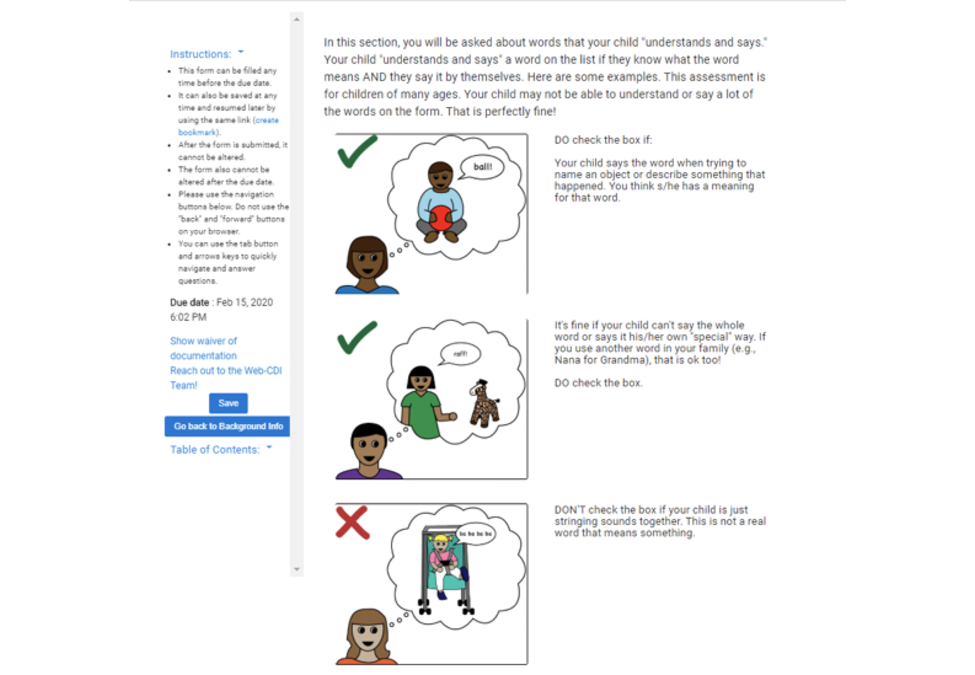
\includegraphics{webcdi_paper_files/figure-latex/pictorial-1.pdf}
\caption{\label{fig:pictorial}Pictorial instructions in the Web-CDI Words and Sentences instrument.}
\end{figure}

\begin{figure}
\centering
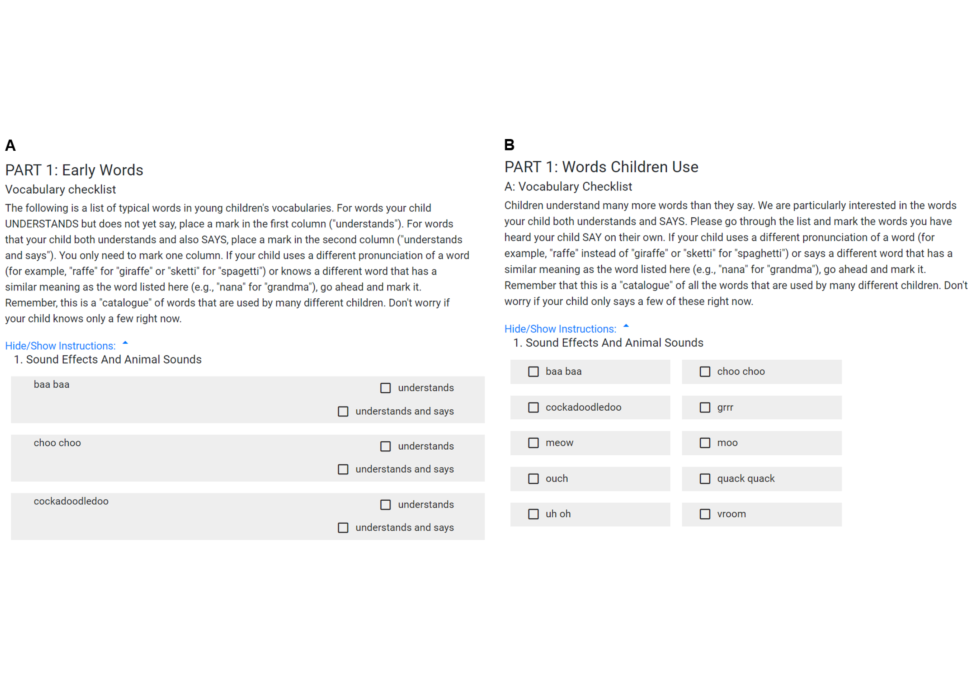
\includegraphics{webcdi_paper_files/figure-latex/firstitems-1.pdf}
\caption{\label{fig:firstitems}(A) Sample items from the American English Words and Gestures form. (B) Sample items from the American English Words and Sentences form.}
\end{figure}

\emph{Instructions.} After completing the first demographics page, participants are provided with detailed instructions that are appropriate for either the Words \& Gestures or Words \& Sentences version (see Figure \ref{fig:pictorial}). In addition, there are more detailed instructions for completing the vocabulary checklist. Unlike the traditional paper versions, instructions on how to properly choose responses are provided both in written and pictorial form. The pictorial instructions (Figure \ref{fig:pictorial}) aim to further increase caregivers' understanding of how to complete the checklist. For example, these instructions clarify that the child's understanding of a word requires them to have some understanding of the object that the word refers to or some aspect of the word's meaning. In addition, caregivers are reassured that \enquote{child-like} forms (e.g., \enquote{raff} for \enquote{giraffe}) or family- or dialect-specific forms (e.g., \enquote{nana} for \enquote{grandma}) are acceptable. Lastly, caregivers are reminded that the child should be able to produce the words \enquote{on their own} and that imitations are not acceptable. These general \enquote{rules of thumb} for completing the form should be familiar to researchers who are distributing the forms to caregivers so they can field any questions that may arise. While this is not possible for certain use-cases (e.g., social media recruitment), these instructions should ideally also be reviewed either in writing (e.g., via email) or verbally (e.g., over the phone), so that these pictured instructions serve merely as a reminder to caregivers when completing the form.

\emph{Completing the instrument.} The majority of the participant's time is spent completing the main sections of the instruments. As shown in Figure \ref{fig:firstitems}, on the American English Words and Gestures form, the vocabulary checklist portion (396 items) asks caregivers to indicate whether their child can \enquote{understand} or \enquote{understand and say} each word; they can also indicate that their child neither understands nor says the word by checking neither box. Additionally, gesture communication and other early milestones are assessed. In the American English Words and Sentences form, the vocabulary checklist (680 items) only asks caregivers to indicate which words their child \enquote{says}. Additional items assess children's production of their three longest sentences, as well as morphological and syntactic development more broadly. All of these items are broken up across multiple screens for easier navigation through the form.

At the completion of the form, a graph is displayed illustrating the proportion of words from each semantic category that the child currently produces or understands. Participants can select to download their own responses. In addition, data from the norming studies are used to estimate the \enquote{hardest} (i.e., most advanced based on previous work on age of acquisition of individual words, Frank et al. (2021)) word that the child currently understands or produces. This feedback to caregivers is intended to provide caregivers with a fun \enquote{thank you} and is intentionally not designed to provide specific feedback about their child's progress relative to other children or any normative standard. The closing page also reminds caregivers that their participation does not constitute a clinical evaluation and that they should contact their pediatrician or primary care physician if they have any concerns about their child's development.

\hypertarget{researcher-interface}{%
\subsection{Researcher interface}\label{researcher-interface}}

One of the main goals of Web-CDI is to provide a unified CDI platform to the child language research community. To that end, researchers request an account by contacting a member of the CDI Advisory Board. Once they have registered an account they can create studies to distribute to participants. One rationale for this personalized registration process is that we ask that researchers allow fully anonymized data from their participants to be shared with the CDI Advisory Board, so that it can be added to Wordbank (\url{http://wordbank.stanford.edu/}; Frank et al., 2017) and shared with broader research community. However, if particular participants indicate in the consent process that they do not want their data to be shared more broadly, then researchers can indicate this in the Web-CDI dashboard to prevent data from specific administrations being contributed to any analyses conducted by the CDI Advisory Board and/or Wordbank.

A study in the context of the Web-CDI system is a set of individual administrations created by a researcher that share certain specifications. Table A1 in the Appendix gives an overview of the customizable features that are available at the study level in Web-CDI. These features are set when creating a study using the \enquote{Create Study} tool, and most of the features can be updated continuously during data collection using the \enquote{Update Study} tool. While some of these features are only particularly relevant to specific use cases (e.g., longitudinal research and social media data collection, described below), others are relevant to all researchers using Web-CDI.

There are currently several CDI forms available for distribution on Web-CDI, including multiple versions of the English WG and WS forms and forms in other languages (see Cross-linguistic Research below). When creating a study, researchers choose one of the forms that they would like to distribute to participants; only one can be used in a given study. Researchers who wish to send multiple forms to participants simultaneously (e.g., those conducting multilingual research) should create multiple studies, each with a single instrument associated with it.

Researchers can download participant data in two formats. Both formatting options output a comma-separated values file with one row per participant; the full data option includes participant-by-item responses, and allows researchers to explore item-level trends, while the summary data option omits item-level data and only provides summary scores and normative information (e.g., total number of words understood/produced, percentile scores by age and gender).

Below, we outline several possible use cases of Web-CDI, as well the features which may facilitate them from a researcher's perspective.

\emph{Individual recruitment.} One possible workflow using Web-CDI is to send unique study URLs to individual participants. Researchers do so by entering numerical participant IDs or by auto-generating a specified quantity of participant IDs, each with its own unique study URL, using the \enquote{Add Participants} tool in the researcher dashboard. New participants can be added on a continual basis so that researchers can adjust the sample size of their study during data collection. Unique links generated for individual participants expire, by default, 14 days after creation, though the number of days before link expiration is adjustable, which may be an important consideration for some researchers depending on their participant populations and specific project timelines. Workflows that involve generating unique links are most suitable for studies which pair the CDI with other measures, or when researchers contact specific participants from an existing database.

\emph{Longitudinal studies.} Web-CDI also facilitates longitudinal study designs in which each participant completes multiple administrations. Researchers wishing to design longitudinal studies can do so by entering a list of meaningful participant IDs using the \enquote{Add Participants} tool in the researcher dashboard. If a certain participant ID is added multiple times, Web-CDI will create multiple unique study URLs in the study dashboard that have the same specified ID. In addition, when creating studies, researchers can select whether they would like the demographics information, vocabulary checklist, or no sections at all to be pre-filled when a participant fills out a repeat administration of the instrument. Unless researchers are interested in cumulative vocabulary counts, it is strongly recommended that they do not use the option to pre-fill the vocabulary checklist portion of the instrument in longitudinal administrations as caregivers should complete the instrument at each time point independently.

\emph{Social media and survey vendors.} Web-CDI contains several features designed to facilitate data collection from social media recruitment or through third-party crowd-sourcing applications and vendors (e.g., Amazon Mechanical Turk, Prolific). First, rather than creating unique survey links for each participant, researchers can also use a single, anonymous link. When a participant clicks the anonymous link, a new administration with a unique subject ID is created in the study dashboard. Additionally, Web-CDI studies have several customizable features that are geared towards anonymous online data collection. For example, researchers can adjust the minimum amount of time a participant must take to fill out the survey before they are able to submit; with a longer minimum time to completion, researchers can encourage a more thorough completion of the survey. Researchers can also ask participants to verify that their information is accurate by checking a box at the end of the survey, and can opt to include certain demographic questions at both the beginning and end of the survey, using response consistency on these redundant items as a check of data quality.

\emph{Paid participation.} If researchers choose to compensate participants directly through the Web-CDI interface, Web-CDI has built-in functionality to distribute redeemable gift codes when a participant reaches the end of the survey. Web-CDI contains several features to facilitate integration with third-party crowdsourcing applications and survey vendors should they choose to handle participant compensation through another platform. For example, when creating studies, researchers can enter a URL to redirect participants to when they reach the end of the survey. Researchers using the behavioral research platform Prolific can configure their study to collect participants' unique Prolific IDs and pre-fill them in the survey.

\emph{Cross-linguistic research.} Web-CDI forms are currently available in English (U.S. American and Canadian), Spanish, French (Quebecois), Hebrew, Dutch and Korean. We are looking to add more language forms to the tool as the paper version of the forms has been adapted into more than 100 different languages and further ongoing adaptations have been approved by the MB-CDI board (\url{http://mb-cdi.stanford.edu/adaptations}).

\hypertarget{system-design}{%
\subsection{System Design}\label{system-design}}

Web-CDI is constructed using open-source software. All of the vocabulary data collected in Web-CDI are stored in a standard MySQL relational database, managed using Django and Python and hosted either by Amazon Web Services or by a European Union (GDPR) compliant server (see below). Individual researchers can download data from their studies through the researcher interface, and Web-CDI administrators have access to the entire aggregate set of data from all studies run with Web-CDI. Website code is available in a GitHub repository \url{https://github.com/langcog/web-cdi}, where interested users can browse, make contributions, and request technical fixes.

\hypertarget{data-privacy-and-gdpr-compliance}{%
\subsection{Data Privacy and GDPR Compliance}\label{data-privacy-and-gdpr-compliance}}

Web-CDI is designed to be compliant with stringent human subjects privacy protections across the world. First, for U.S. users, we have designed Web-CDI based on the United States Department of Health and Human Services \enquote{Safe Harbor} Standard for collecting protected health information as defined by the Health Insurance Portability and Accountability Act (HIPAA). In particular, participant names are never collected, birth dates are used to calculate age in months (with no decimal information) but never stored, and geographic zip codes are trimmed to the first 3 digits. Because of the architecture of the site, even though participants enter zip codes and dates of birth, these are never transmitted in full to the Web-CDI server. Since no identifying information is being collected by the Web-CDI system, this feature ensures that Web-CDI can be used by United States labs without a separate Institutional Review Board agreement between users labs and Web-CDI (though of course researchers using the site will need Institutional Review Board approval of their own research projects).\footnote{Issues of de-identification and re-identifiability are complex and ever changing. In particular, compliance with DHHS \enquote{safe harbor} standards does not in fact fully guarantee the impossibility of statistical re-identification in some cases and if potential users have questions, we encourage them to consult with an Institutional Review Board.}

In the European Union (EU), research data collection and storage is governed by the Generalized Data Protection Regulation (GDPR) and its local instantiation in the legal system of the member states. Some of the questions on the demographic form contain information that may be considered sensitive (e.g., information about children's developmental disorders), and in some cases, the possibility of linking this sensitive information to participant IDs exists, particularly when researchers draw on local databases that contain full names and addresses for recruitment and contacting. As a result, issues regarding GDPR compliance arise when transferring data outside the EU, namely to Amazon Web Services servers housed in the United States. Following GDPR regulations, these issues would make a data sharing agreement between data collectors and Amazon Web Services necessary. In addition, all administrators who can access the collected data would have to enter such an agreement, which needs updating whenever personnel changes occur. To overcome these hurdles, and in consultation with data protection officers, we opted to leverage the local technical expertise and infrastructure to set up a sister site housed on GDPR-compliant servers, currently available at \url{http://webcdi.mpi.nl}. This site is updated synchronously with the main Web-CDI website to ensure a consistent user experience and access to the latest features and improvements. This site has been used in 135 successful administrations so far and is the main data collection tool for an ongoing norming study in the Netherlands. We are further actively advertising the option to use the European site to other labs who are following GDPR guidelines and are planning adaptations to multiple European languages, where copyright allows.

We now turn to an overview of the data collected thus far using Web-CDI. First, we examine the full sample of all of the Web-CDI administrations collected as of autumn 2020 (Dataset 1); we then focus in on a specific subset of Dataset 1 which is comprised of data from recent efforts to oversample non-white, less highly-educated U.S. participants (Dataset 2). Across both datasets, we show that general trends from prior research on vocabulary development are replicated using Web-CDI, and we discuss the potential for using Web-CDI to collect vocabulary development data from diverse communities online.

\hypertarget{dataset-1-full-current-web-cdi-usage}{%
\section{Dataset 1: Full Current Web-CDI Usage}\label{dataset-1-full-current-web-cdi-usage}}

\begin{table}

\caption{\label{tab:unnamed-chunk-1}Exclusions from Dataset 1: full Web-CDI sample}
\centering
\resizebox{\linewidth}{!}{
\begin{tabular}[t]{>{\raggedright\arraybackslash}p{2.4in}>{\raggedright\arraybackslash}p{1in}>{\raggedright\arraybackslash}p{1in}>{\raggedright\arraybackslash}p{1in}>{\raggedright\arraybackslash}p{1in}}
\toprule
\textbf{Exclusion} & \textbf{WG exclusions} & \textbf{\% of full WG sample excluded} & \textbf{WS exclusions} & \textbf{\% of full WS sample excluded}\\
\midrule
Not first administration & 163 & 5.68\% & 444 & 12.35\%\\
Premature or low birthweight & 37 & 1.29\% & 67 & 1.86\%\\
Multilingual exposure & 449 & 15.66\% & 492 & 13.69\%\\
Illnesses/Vision/Hearing & 191 & 6.66\% & 203 & 5.65\%\\
Out of age range & 88 & 3.07\% & 200 & 5.56\%\\
Completed survey too quickly & 363 & 12.66\% & 236 & 6.57\%\\
System error in word tabulation & 1 & 0.03\% & 4 & 0.11\%\\
Total exclusions & 1292 & 45\% & 1646 & 46\%\\
\bottomrule
\end{tabular}}
\end{table}

In this section, we provide some preliminary analyses of Dataset 1 which consists of the full sample of American English Web-CDI administrations collected before autumn 2020. At time of writing, researchers from 15 universities in the United States have collected over 5,000 administrations of the American English CDI using Web-CDI since it was launched in late 2017, with 2,868 administrations of the WG form before exclusions and 2,868 administrations of the WS form before exclusions. We excluded participants from the subsequent analyses based on a set of stringent criteria intended for the creation of future normative datasets. We excluded participants if it was not their first administration of the survey; if they were born prematurely or had a birthweight under 5.5 lbs (\textless{} 2.5 kg); reported more than 16 hours of exposure to a language other than English per week on average (amounting to \textgreater{} 10\% exposure to English); had serious vision impairments, hearing deficits or other developmental disorders or medical issues\footnote{Exclusions on the basis of child health were decided on a case-by-case basis by author V.M. in consultation with Philip Dale, Donna Thal, and Larry Fenson.}; completed the survey unrealistically quickly (defined here as in fewer than 8.5 minutes)\footnote{This timing criterion was chosen by authors B.D. and V.M. during recent online data collection as a lenient cutoff, i.e., one that errs on the side of including, rather than excluding, participants; on paper-based forms, caregivers are told the test generally takes 20-40 minutes. We noted that in early rounds of recent data collection, most participants who completed the survey in less than 8.5 minutes reported floor-level vocabulary scores regardless of age.}; or were outside of the correct age range for the survey. The exclusion criteria we used were designed to be generally comparable with those used in Fenson et al. (2007), who adopted stringent criteria to establish vocabulary norms that reflect typically developing children's vocabulary trajectories. A complete breakdown of the number of participants excluded on each criterion is in Table 1. Of the completed WG forms, 1,292 were excluded, leading to a final WG sample size of 1,576 administrations, and 920 WS administrations were excluded, leading to a final WS sample size of 1,948.

\begin{figure}
\centering
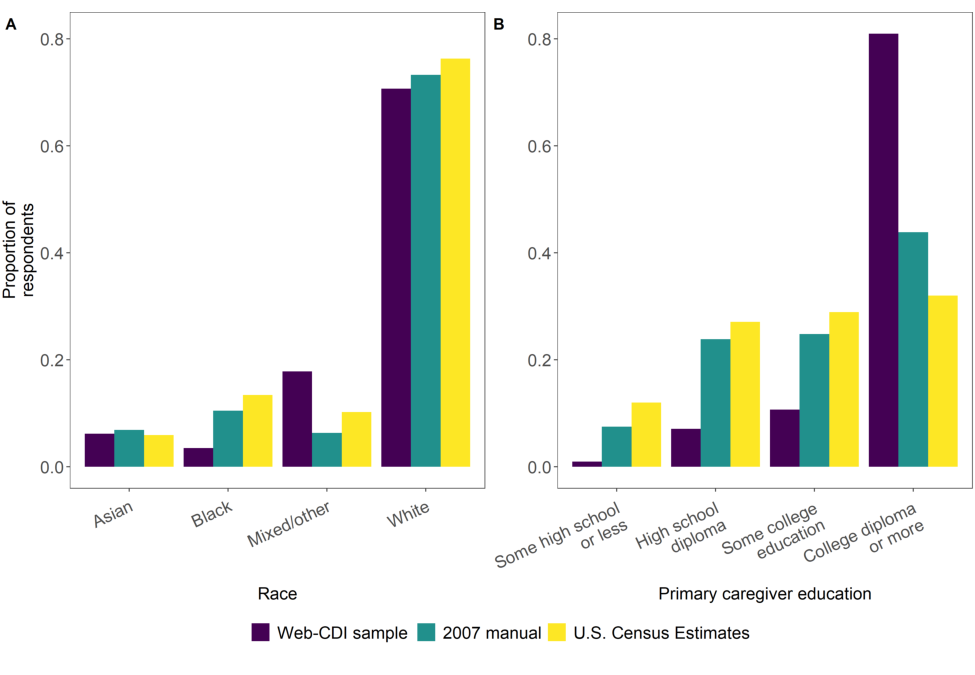
\includegraphics{webcdi_paper_files/figure-latex/demobarfig-1.pdf}
\caption{\label{fig:demobarfig}Proportion of respondents plotted by child race (A) and educational level of primary caregiver (B) from full Web-CDI sample (Dataset 1) to date (N = 3,524), compared with norming sample demographics from Fenson (2007). Latinx participants can be of any race and are thus not represented as a separate category here.}
\end{figure}

\hypertarget{demographic-distribution-and-exclusions}{%
\subsection{Demographic distribution and exclusions}\label{demographic-distribution-and-exclusions}}

Figure \ref{fig:demobarfig} shows the distribution of participant ethnicities in Dataset 1 as compared with previously reported numbers in a large scale norming study of the paper-based CDI form by Fenson et al. (2007). White participants still comprised nearly three quarters of the Web-CDI sample, while a higher proportion of participants report mixed ethnic identification as compared to the 2007 norms. Few participants identified as Hispanic/Latinx: 6.5\% of WG participants and 5.1\% of WS participants reported Hispanic or Latinx heritage. The low percentage of Hispanic/Latinx participants was due in part to our exclusion of children with substantial exposure to languages other than English: before exclusions, 8.4\% of WG participants were Hispanic/Latinx, and 8.1\% of WS participants were Hispanic/Latinx.

Participants' educational attainment level was similarly skewed. Over 80\% of children in Dataset 1 came from families with college-educated mothers compared to 43\% from the same group in the 2007 norms (Figure \ref{fig:demobarfig}). Furthermore, less than 1\% of participants report a primary caregiver education level less than a high school degree, compared to 7\% from the same group in the 2007 norms. The overrepresentation of white Americans with high levels of education attainment in this sample points to a general challenge encountered in vocabulary development research, which we return to when we detail our efforts to recruit more diverse participants.

\hypertarget{results}{%
\subsection{Results}\label{results}}

\begin{figure}
\centering
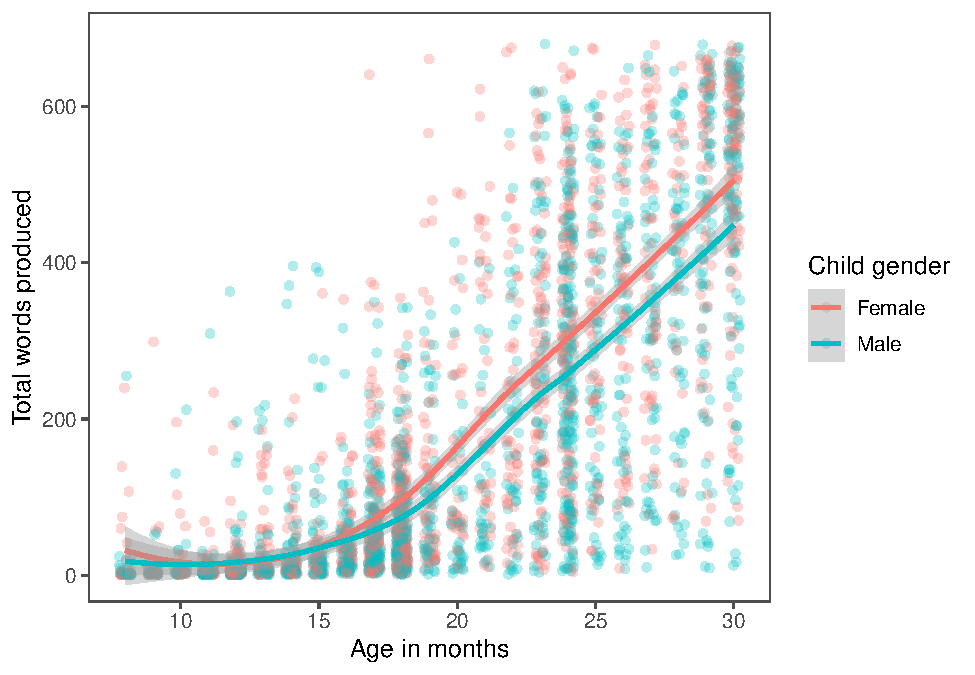
\includegraphics{webcdi_paper_files/figure-latex/genderfig-1.pdf}
\caption{\label{fig:genderfig}Individual children's vocabulary production scores from Dataset 1 (entire Web-CDI sample) plotted by children's age and gender (both WG and WS, N = 3,513, with 1,674 girls). Lines are locally weighted regressions (LOESS) with associated 95\% confidence interval. Children with a different or no reported gender (N = 11) are omitted here.}
\end{figure}

Although the CDI instruments include survey items intended to measure constructs other than vocabulary size, such as gesture, sentence production and grammar, we focus exclusively on the vocabulary measures here. Across both the WG and WS measures, Dataset 1 shows greater reported vocabulary comprehension and production for older children. Moreover, data from both the WG and WS measures in Dataset 1 replicate a subtle but reliable pattern such that female children tend to have slightly larger vocabulary scores than male children across the period of childhood assessed in the CDI forms (Frank et al., 2021), though in these data this difference does not appear until around 18 months (Figure \ref{fig:genderfig}).

\begin{figure}
\centering
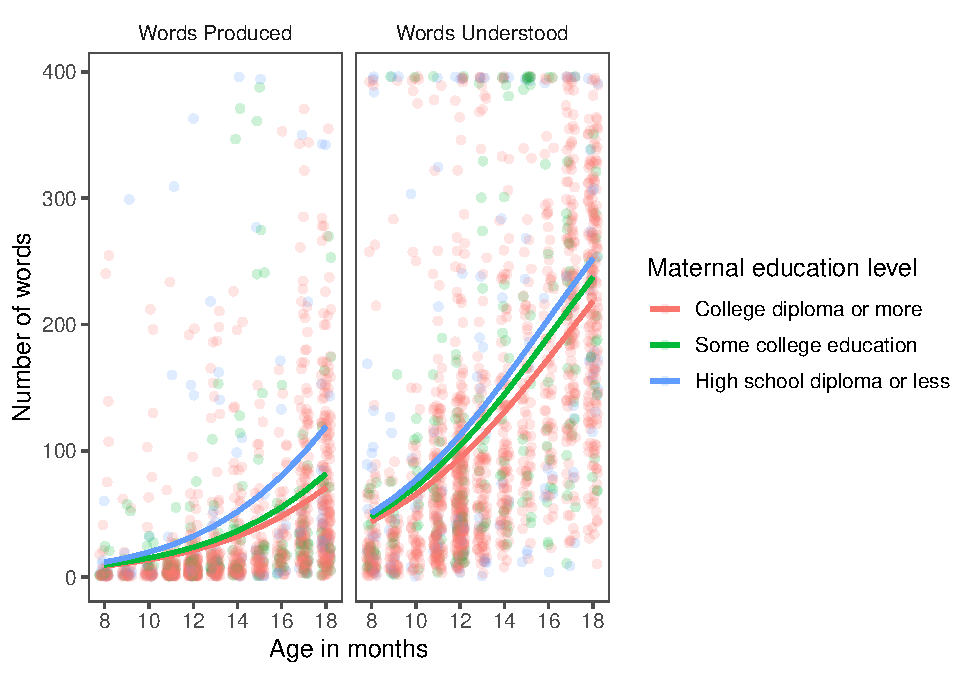
\includegraphics{webcdi_paper_files/figure-latex/wgglm-1.pdf}
\caption{\label{fig:wgglm}Individual children's word production (left panel) and comprehension (right panel) scores from Dataset 1 (full Web-CDI sample) plotted by age and primary caregiver's level of education (binned into \enquote{High school diploma or less}, \enquote{Some college education}, and \enquote{College diploma or more}) as reported in the sample of Words and Gestures Web-CDI administrations collected as of November 2020 (N = 1,576). Curves show generalized linear models fits.}
\end{figure}

\begin{figure}
\centering
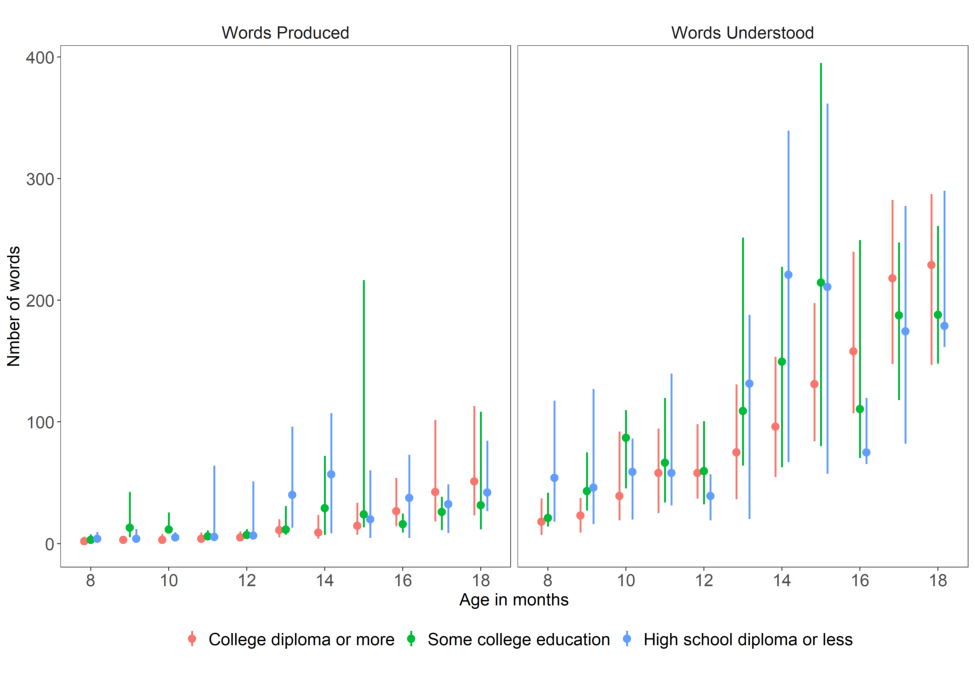
\includegraphics{webcdi_paper_files/figure-latex/wgmedfig-1.pdf}
\caption{\label{fig:wgmedfig}Median vocabulary production (left) and comprehension (right) scores from Dataset 1 (full Web-CDI sample) by age and primary caregiver's level of education attainment on the WG form. Lines indicate span between first and third quartiles for each age.}
\end{figure}

\begin{figure}
\centering
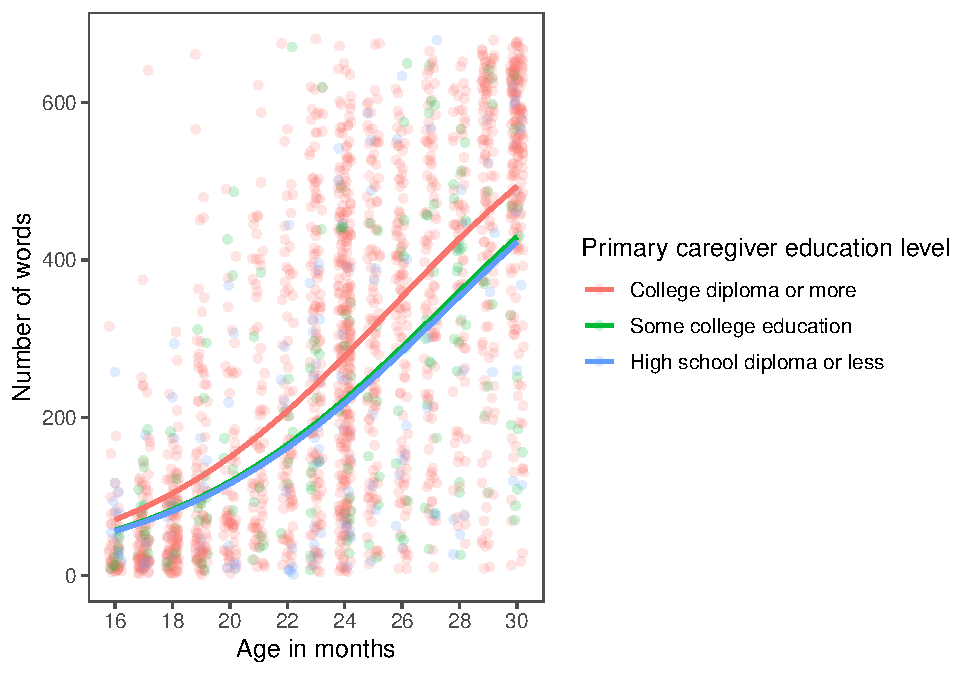
\includegraphics{webcdi_paper_files/figure-latex/wsglm-1.pdf}
\caption{\label{fig:wsglm}Individual children's vocabulary production scores from Dataset 1 (full Web-CDI sample) plotted by children's age and primary caregiver education level of primary caregiver education as reported in the sample of Words and Sentences Web-CDI administrations collected as of November 2020 (N = 1,948). Curves show generalized linear models fits.}
\end{figure}

On the WG form, respondents' reports of children's vocabulary comprehension and production both increased with children's age (Figure \ref{fig:wgglm}). We replicate overall patterns found by Feldman et al. (2000) in that, on both the \enquote{Words Understood} and \enquote{Words Produced} measures, vocabulary scores were slightly negatively correlated with primary caregivers' education level, such that those caregivers without any college education reported higher vocabulary scores on both scales. A linear regression model with robust standard errors predicting comprehension scores with children's age and primary caregivers' education level (binned into categories of \enquote{High school diploma or less}, \enquote{Some college education} and \enquote{College diploma or more\footnote{"High school diploma or less" corresponds to 12 or fewer years of education; "Some college" corresponds to 13 - 15 years of education; "College diploma or more" refers to 16 or more years of education.}}) as predictors shows main effects of both age (\(\beta\) = 19.89, \(p\) \textless{} 0.001) and caregiver primary education (\(\beta_{high school}\) = 29.59, \(p\) = 0.01). Similarly, a linear regression model with robust standard errors predicting production scores by children's age and primary caregivers' education level shows main effects of age (\(\beta\) = 7.82, \(p\) \textless{} 0.001) and caregiver primary education (\(\beta_{high school}\) = 28.86, \(p\) = 0.002). These analyses were not preregistered, but generally follow the analytic strategy in Frank et al. (2021); additionally, we fit linear models with robust standard errors to account for heteroskedasticity in the data (Astivia \& Zumbo, 2019).

The pattern of results seen in the WG subsample of Dataset 1 is consistent with prior findings indicating that respondents with lower levels of education attainment report higher vocabulary comprehension and production on the CDI-WG form (Feldman et al., 2000; Fenson et al., 1994). Although caregivers with lower levels of education attainment report higher mean levels of vocabulary production and comprehension, median vocabulary scores (which are more robust to outliers) show no clear pattern of difference across primary caregiver education levels (Figure \ref{fig:wgmedfig}). This discrepancy between the regression effects and a group-median analysis suggests that the regression effects described previously are driven in part by differential interpretation of the survey items, such that a few caregivers with lower levels of education attainment are more liberal in reporting their children's productive and comprehensive vocabularies, especially for the youngest children, driving up the mean scores for this demographic group.

Vocabulary production scores on the WS form show the expected pattern of increase with children's age in months; in addition, scores replicate the trend reported in Feldman et al. (2000) and Frank et al. (2021) such that primary caregiver education is positively associated with children's reported vocabulary size (Figure \ref{fig:wsglm}). Because representation of caregivers without a high school diploma is scarce (N = 18 out of a sample of 1,948), interpretation of the data from this group is constrained. Nevertheless, as shown in Figure \ref{fig:wsglm}, a small but clear positive association between primary caregiver education and vocabulary score exists such that college-educated caregivers report higher vocabulary scores than those of any other education level. The implications from these data converge with previous findings which indicate that parental education levels, often used as a metric of a family's socioeconomic status, are related to children's vocabulary size through early childhood.

\hypertarget{discussion-dataset-1}{%
\subsection{Discussion: Dataset 1}\label{discussion-dataset-1}}

In general, the full sample of Web-CDI data after exclusions (Dataset 1) replicates previous norming datasets used with the standard paper-and-pencil form of the MB-CDI. We find that vocabulary scores grow with age and that females hold a slight advantage over males in early vocabulary development. Moreover, Dataset 1 replicates a previously documented relationship between primary caregiver education level and vocabulary scores: on the WG form, primary caregiver education shows a slight negative association with vocabulary scores, whereas the trend is reversed in the WS form. Taken together, these data illustrate that Web-CDI and the standard paper-and-pencil form of the CDI give similar results, and thus that Web-CDI can be used as a valid alternative to the paper format.

The data discussed above have stemmed from efforts by many researchers across the United States whose motivations for using the Web-CDI vary. As a result, they reproduce many of the biases of standard U.S. convenience samples. In the next section, we describe in more detail our recent efforts to use the Web-CDI to collect vocabulary development data from traditionally underrepresented participant populations in the United States, attempting to counteract these trends.

\hypertarget{dataset-2-using-web-cdi-to-collect-data-from-diverse-u.s.-based-communities}{%
\section{Dataset 2: Using Web-CDI to Collect Data from Diverse U.S.-based Communities}\label{dataset-2-using-web-cdi-to-collect-data-from-diverse-u.s.-based-communities}}

Despite the large sample sizes we collected in the previous section, Dataset 1 is, if anything, even more biased towards highly-educated white families than previous datasets collected using the paper-and-pencil form. How can we recruit more diverse samples to remedy this issue? Here, we discuss and analyze Dataset 2, which consists of those administrations from Dataset 1 which were part of recent data-collection efforts (within the past year and a half) that were specifically aimed towards exploring the use of online recruitment as a potential way to collect more diverse participant samples than are typical in the literature. In other words, the following data from Dataset 2 were included in the previous discussion and analysis of Dataset 1, but we examine them separately here to give special attention to the issue of collecting diverse samples online.

While understanding that the performance of standard measurement tools like the CDI among multilinguals is of immense import to the field of vocabulary development research (Gonzalez et al., in prep; Floccia et al., 2018; De Houwer, 2019), we focused in Dataset 2 only on vocabulary development in monolingual children, because collecting data from multilingual populations introduces additional methodological considerations (e.g., how to measure exposures in each language) that are not the focus of our work here. However, it will be imperative in future to collect large-scale datasets of vocabulary data in bilingual children, both to better calibrate standard tools such as the CDI, as well as to reduce the bias towards monolingual families in the existing literature on measuring vocabulary development.

\hypertarget{online-data-collection}{%
\subsection{Online data collection}\label{online-data-collection}}

Online recruitment methods, such as finding participants on platforms such as Amazon Mechanical Turk, Facebook and Prolific, represent one possible route towards assembling a large, diverse sample to take the Web-CDI. These methods allow researchers to depart from their typical geographical recruitment area much more easily than with paper-and-pencil administration. Online recruitment strategies for vocabulary development data collection have been used in the United Kingdom (Alcock, Meints, \& Rowland, 2020), but their usage in the U.S. context remains, to our knowledge, rare. In a series of data collection efforts, we used Web-CDI as a tool to explore these different channels of recruitment.

\begin{figure}
\centering
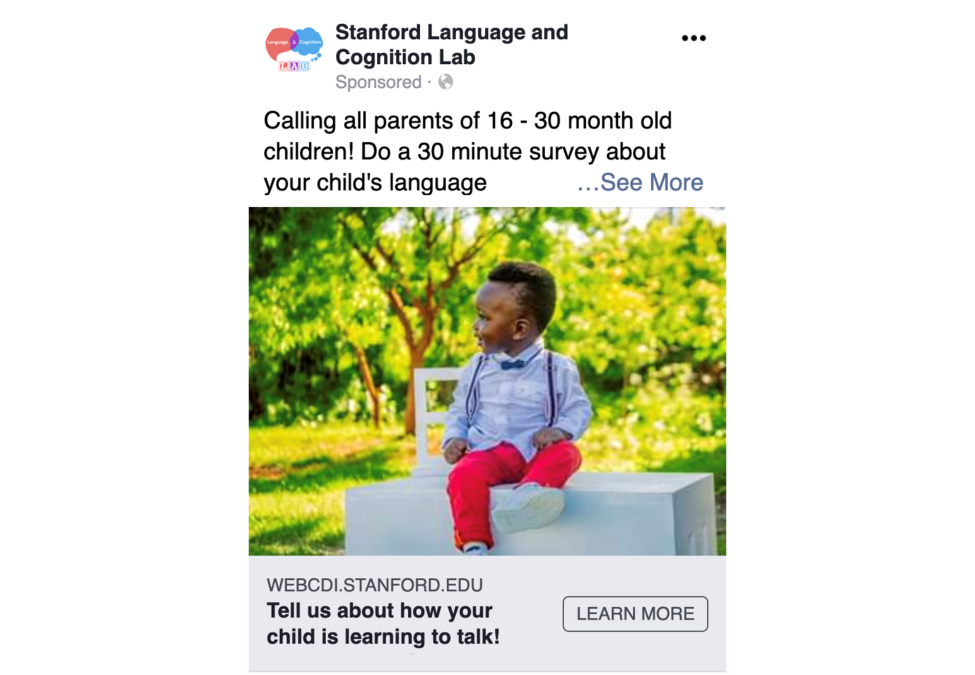
\includegraphics{webcdi_paper_files/figure-latex/facebookad-1.pdf}
\caption{\label{fig:facebookad}Example Facebook advertisement in Phase 1 of recent data collection.}
\end{figure}

\begin{table}

\caption{\label{tab:unnamed-chunk-8}Exclusions from Dataset 2: recent data collection using Facebook and Prolific.}
\centering
\resizebox{\linewidth}{!}{
\begin{tabular}[t]{>{\raggedright\arraybackslash}p{2.4in}>{\raggedright\arraybackslash}p{1in}>{\raggedright\arraybackslash}p{1in}>{\raggedright\arraybackslash}p{1in}>{\raggedright\arraybackslash}p{1in}}
\toprule
\textbf{Exclusion} & \textbf{WG exclusions} & \textbf{\% of full WG sample excluded} & \textbf{WS exclusions} & \textbf{\% of full WS sample excluded}\\
\midrule
Not first administration & 0 & 0.00\% & 0 & 0.00\%\\
Premature or low birthweight & 7 & 2.53\% & 1 & 0.33\%\\
Multilingual exposure & 18 & 6.50\% & 23 & 7.62\%\\
Illnesses/Vision/Hearing & 4 & 1.44\% & 4 & 1.32\%\\
Out of age range & 1 & 0.36\% & 26 & 8.61\%\\
Completed survey too quickly & 132 & 47.65\% & 122 & 40.40\%\\
System error in word tabulation & 0 & 0.00\% & 0 & 0.00\%\\
Total exclusions & 162 & 58\% & 176 & 58\%\\
\bottomrule
\end{tabular}}
\end{table}

Dataset 2 consists of data that were collected in two phases. In the first phase, we ran advertisements on Facebook which were aimed at non-white families based on users' geographic locations (e.g., targeting users living in majority-Black cities) or other profile features (e.g., ethnic identification, interest in parenthood-related topics). Advertisements consisted of an image of a child and a caption informing Facebook users of an opportunity to fill out a survey on their child's language development and receive an Amazon gift card (Figure \ref{fig:facebookad}). Upon clicking the advertisement, participants were redirected to a unique administration of the Web-CDI, and they received \$5 upon completing the survey. This open-ended approach to recruitment offered several advantages, namely that a wide variety of potential participants from specific demographic backgrounds can be reached on Facebook. However, we also received many incomplete or otherwise unusable survey administrations, either from Facebook users who clicked the link and decide not to participate, or those who completed the survey in an extremely short period of time (over half of all completed administrations, Table 2).

In the second phase, we used the crowdsourcing survey vendor Prolific (\url{http://prolific.co}) in the hopes that some of the challenges encountered with Facebook recruitment would be addressed. Prolific allows researchers to create studies and post them to individuals who are in the platform's participant database, each of whom is assigned a unique alphanumeric \enquote{Prolific ID}. Importantly, Prolific maintains detailed demographic information about participants, allowing researchers to specify whom they would like to complete their studies. Prolific further has a built-in compensation infrastructure that handles monetary payments to participants, eliminating the need to disburse gift cards through Web-CDI.

In the particular case of Web-CDI, the demographic information needed to determine whether an individual was eligible to complete our survey (e.g., has a child in the correct age range, lives in a monolingual household, etc.) was more specific than the information that Prolific collects about their participant base. We therefore used a brief pre-screening questionnaire to generate a list of participants who were eligible to participate, and subsequently advertised the Web-CDI survey to those participants. Given that we were interested only in reaching participants in the United States who were not white or who did not have a college diploma, our data collection efforts only yielded a sample that was small (N = 71) but much more thoroughly screened than that which we could obtain on Facebook.

Across both phases (Facebook and Prolific recruitment), we used the same exclusion criteria as in the full Web-CDI sample to screen participants. A complete tally of all excluded participants is shown in Table 2. In both the WG and WS surveys, exclusion rates in Dataset 2 were high, amounting to 58\% of participants who completed the survey. The high exclusions rates were notably driven by an accumulation of survey administrations which participants completed very quickly (in these analyses, defined as a completion taking less than 8.5 minutes). Many of the survey administrations excluded for fast completion had missing demographic information reported: Among WG participants excluded for too-fast completions, 93\% did not report ethnicity, and among WS participants excluded for the same reason, 97\% did not report ethnicity. Absence of these data prevents us from making conclusions about the origin or demographic profile of administrations that were excluded. After exclusions, full sample size in Dataset 2 was N = 115 WG completions and N = 126 WS completions.

\begin{figure}
\centering
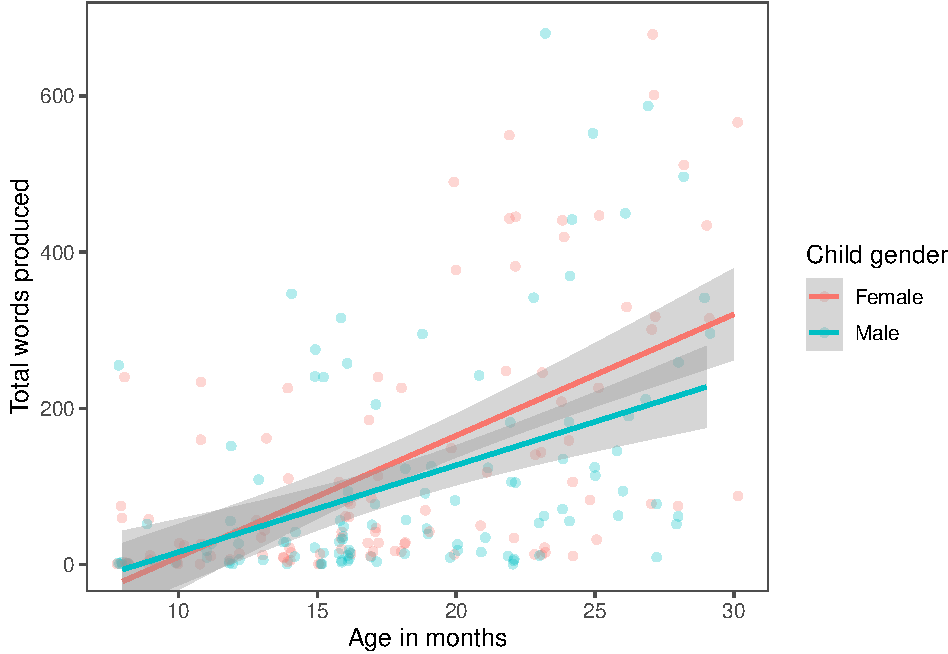
\includegraphics{webcdi_paper_files/figure-latex/genderses-1.pdf}
\caption{\label{fig:genderses}Individual children's vocabulary production scores from Dataset 2 (recent data collection efforts) plotted by children's age and gender (both WG and WS, N = 238, with 116 girls). Lines are best linear fits with associated 95\% confidence intervals. Children with a different or no reported gender (N = 3) are omitted here.}
\end{figure}

\begin{figure}
\centering
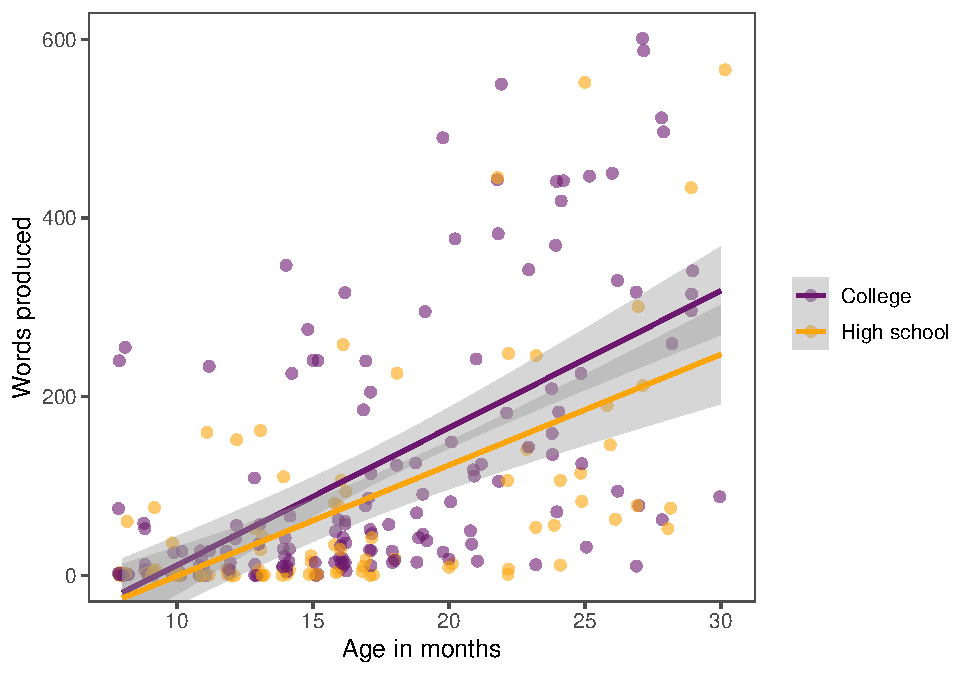
\includegraphics{webcdi_paper_files/figure-latex/momedses-1.pdf}
\caption{\label{fig:momedses}Individual children's vocabulary production scores from Dataset 2 (recent data collection efforts) plotted by age and level of primary caregiver education, binned into those with a high school diploma or less education and those with some college education or a college diploma (N = 241). Lines show best linear fits and associated 95\% confidence intervals.}
\end{figure}

\begin{figure}
\centering
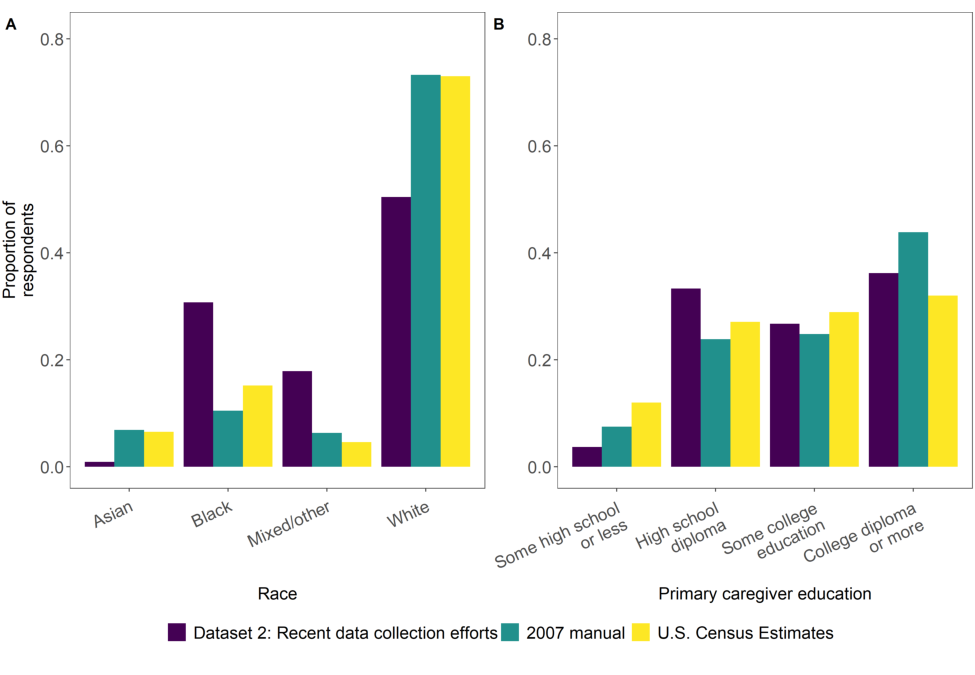
\includegraphics{webcdi_paper_files/figure-latex/demobarses-1.pdf}
\caption{\label{fig:demobarses}Proportion of respondents plotted by child race (A) and educational level of primary caregiver (B) from Dataset 2, recent data collection efforts aimed towards oversampling non-white, less highly-educated families (N = 241), compared with norming sample demographics from Fenson (2007). Latinx participants can be of any race and are thus not represented as a separate category here.}
\end{figure}

The results from Dataset 2 show overall similar patterns to the full Web-CDI sample in several regards. Word production scores from both the WG and WS administrations reflect growing productive vocabulary across the second and third years, with a very small gender effect such that female children's vocabularies are higher across age than males' (Figure \ref{fig:genderses}). The relationship between caregivers' reported levels of education and child's vocabulary score is not as clear as it is in the full Web-CDI sample (Figure \ref{fig:momedses}); however, children of college-educated caregivers reported generally higher vocabulary scores across age than did children of caregivers without any college degree. These patterns suggest that our data show similar general patterns to other CDI datasets with other populations (Frank et al., 2021).

Importantly, Dataset 2 showed a substantial improvement in reaching non-white or less highly-educated participants. After exclusions, Dataset 2 has a higher proportion of non-white participants than Dataset 1 (the overall Web-CDI sample) and the norms established by Fenson et al. (2007) (Figure \ref{fig:demobarses}). Black participants in particular showed a marked increase in representation, from 10.5\% in the 2007 norms to 30.9\% in Dataset 2, while the proportion of white participants decreased from 73.3\% in the 2007 norms to 50.2\% in Dataset 2. Representation on the basis of families' reported primary caregiver education also improved (Figure \ref{fig:demobarses}). Participants with only a high school diploma accounted for 31.5\% of Dataset 2 as compared to 23.8\% in the 2007 norms, and representation of those with a college diploma or more education decreased from 43.8\% in the 2007 norms to 36.5\% in Dataset 2.

\hypertarget{discussion-dataset-2}{%
\subsection{Discussion: Dataset 2}\label{discussion-dataset-2}}

The results from Dataset 2 indicate that Web-CDI could be a promising platform to collect vocabulary development data in non-white and communities with lower levels of education attainment when paired with online recruitment methods that yield legitimate, representative participant samples. These data do, however, convey clear limitations of our approach. Perhaps most conspicuously, more than half of completed administrations in this sample had to be excluded, in many cases because the information provided by participants appeared rushed or incomplete: over 40\% of administrations were completed in fewer than 8.5 minutes, and of these quick completions, well over 90\% were missing demographic information that is rarely missing in other administrations of the form. Determining the precise reasons for the high exclusion rate, and how (if at all) this (self-)selection may bias data reflecting demographic trends in vocabulary development, requires a more thorough assessment of who is submitting hastily-completed forms. Such an assessment is beyond the scope of the current study. However, all respondents who got to the end of the form were compensated regardless of how thoroughly they completed it, creating the possibility that some participants who clicked the anonymous link may not have been members of the population of interest, but rather were other individuals motivated by compensation.

Additionally, the exclusion rates described previously only provide information on those participants who did, at some point, submit a completed form, but many individuals clicked the advertisement link and did not subsequently continue on to complete the form. Without an in-depth exploration of who is clicking the link and why they might choose not to continue, we cannot draw conclusions about the representativeness of the sample in Dataset 2 with regards to the communities we would like to include in our research. As such, a more thorough understanding of how users from different communities respond to various recruitment and sampling methods is needed in future work in order to draw conclusions about demographic trends above and beyond those already established in the literature.

Similarly, participants in Dataset 2 were recruited through a targeted post on social media, a technique that is considerably more anonymous than recruitment strategies which entail face-to-face or extended contact between researchers and community members. Online recruitment methods may not be suitable for all communities, especially when researchers ask participants to report potentially sensitive information about the health, developmental progress, ethnicity and geographic location of their children (even when such information is stored anonymously). Our goal here was to assess whether general trends in past literature could be recovered using such an online strategy, but future research should take into account that other more personal methods of recruitment, such as more direct community outreach or liaison contacts, may improve participants' experiences and their willingness to engage with the study.

Finally, a significant limitation of the data collection process in Dataset 2 is that many people in the population of interest - particularly lower-income families - do not have reliable internet access. Having participants complete the Web-CDI on a mobile device may alleviate some of the issues caused by differential access to Wi-Fi, since the vast majority of American adults own a smartphone (Center, n.d.). Accordingly, improving Web-CDI's user experience on mobile platforms will be an important step towards ensuring that caregivers across the socioeconomic spectrum can easily complete the survey. For smartphone users on pay-as-you-go plans, who may be reluctant to use phone data to complete a study, a possible solution could be compensating participants for the amount of \enquote{internet time} they incurred completing the form.

\hypertarget{general-discussion-and-conclusions}{%
\section{General Discussion and Conclusions}\label{general-discussion-and-conclusions}}

In this paper, we presented Web-CDI, a comprehensive online interface for researchers to measure children's vocabulary by administering the MacArthur-Bates Communicative Development Inventories family of parent-report instruments. Web-CDI provides a convenient researcher management interface, built-in data privacy protections, and a variety of features designed to make both longitudinal and social-media sampling easy. To date, over 3,500 valid administrations of the WG and WS forms have been collected on Web-CDI from more than a dozen researchers in the United States after applying strict exclusion criteria derived from previous norming studies (Fenson et al., 2007, 1994). Our analysis of Dataset 1 shows that demographic trends from previous work using the paper-and-pencil CDI form are replicated in data gleaned from Web-CDI, suggesting that the Web-CDI is a valid alternative to the paper form and captures similar results.

Many research laboratories, not only in the United States but around the world, collect vocabulary development data using the MacArthur-Bates CDI. With traditional paper-based forms, combining insights from various research groups can prove challenging, as each group may have slightly different ways of formatting and managing data from CDI forms. By contrast, if all of these groups' data come to be stored in a single repository with a consistent database structure, data from disparate sources can easily be collated and analyzed in a uniform fashion. As such, a centralized repository such as Web-CDI provides a streamlined data-aggregation pipeline that facilitates cross-lab collaborations, multisite research projects and the curation of large datasets that provide more power to characterize the vast individual differences present in children's vocabulary development.

Beyond the goal of simply getting more data, we hope that Web-CDI can advance efforts to expand the reach of vocabulary research past convenience samples into diverse communities. A key question in the field of vocabulary development concerns the mechanisms through which sociodemographic variables, such as race, ethnicity, income and education are linked to group differences in vocabulary outcomes. Large, population-representative samples of vocabulary development data are needed to understand these mechanisms, but most research to date (including the full sample of Web-CDI administrations) oversamples white participants and those with advanced levels of education.

We explored the use of Web-CDI as part of a potential strategy to collect data from non-white and less highly-educated communities in two phases (Dataset 2). Several overall patterns emerged which we expected: vocabulary scores grew with age, providing a basic validity check of the Web-CDI measure; females held a slight advantage in word learning over males; and children of caregivers with a college education showed slightly higher vocabulary scores. Nonetheless, the insights from these data, while aligned with past norming studies, are necessarily constrained by several features of our method.

Web-based data collection can capture useful information about vocabulary development from diverse communities, but future research will need to examine which sampling methods can yield accurate, population-representative data that can advance our understanding of the link between sociodemographic variation and variation in language outcomes.

\hypertarget{ethics-statement}{%
\section{Ethics statement}\label{ethics-statement}}

Data collected in the United States for this project are anonymized according to guidelines set forth by the United States Department of Health and Human Services. Data collection at Stanford University was approved by the Stanford Institutional Review Board (IRB), protocol 20398.

\hypertarget{open-access-materials}{%
\section{Open access materials}\label{open-access-materials}}

Data, analytic code and manuscript materials are available on the Open Science Framework at \url{https://osf.io/nmdq4/}.

\hypertarget{author-contributions}{%
\section{Author contributions}\label{author-contributions}}

\begin{itemize}
\tightlist
\item
  Conceptualization: Benjamin deMayo, Danielle Kellier, Mika Braginsky, Caroline Rowland, Michael Frank and Virginia Marchman.
\item
  Data Curation: Benjamin deMayo, Danielle Kellier and Virginia Marchman.
\item
  Formal Analysis: Benjamin deMayo.
\item
  Funding Acquisition: Caroline Rowland and Michael Frank.
\item
  Investigation: Benjamin deMayo and Virginia Marchman.
\item
  Methodology: Benjamin deMayo, Danielle Kellier, Michael Frank and Virginia Marchman.
\item
  Project Administration: Caroline Rowland, Michael Frank and Virginia Marchman.
\item
  Software: Danielle Kellier, Mika Braginsky, Christina Bergmann and Cielke Hendriks.
\item
  Supervision: Caroline Rowland, Michael Frank and Virginia Marchman.
\item
  Visualization: Benjamin deMayo.
\item
  Writing - Original Draft Preparation: Benjamin deMayo, Michael Frank and Virginia Marchman.
\item
  Writing - Review \& Editing: Benjamin deMayo, Danielle Kellier, Mika Braginsky, Christina Bergmann, Cielke Hendriks, Michael Frank and Virginia Marchman.
\end{itemize}

\hypertarget{software-used}{%
\section{Software used}\label{software-used}}

R (Version 4.0.2; R Core Team, 2020) and the R-packages \emph{broman} (Version 0.71.6; Broman, 2020), \emph{cowplot} (Version 1.1.0; Wilke, 2020), \emph{dplyr} (Version 1.0.2; Wickham et al., 2020), \emph{estimatr} (Version 0.26.0; Blair, Cooper, Coppock, Humphreys, \& Sonnet, 2020), \emph{forcats} (Version 0.5.0; Wickham, 2020a), \emph{fs} (Version 1.5.0; Hester \& Wickham, 2020), \emph{ggplot2} (Version 3.3.2; Wickham, 2016), \emph{here} (Version 0.1; Müller, 2017), \emph{kableExtra} (Version 1.3.1; Zhu, 2020), \emph{papaja} (Version 0.1.0.9997; Aust \& Barth, 2020), \emph{purrr} (Version 0.3.4; Henry \& Wickham, 2020), \emph{readr} (Version 1.4.0; Wickham \& Hester, 2020), \emph{scales} (Version 1.1.1; Wickham \& Seidel, 2020), \emph{stringr} (Version 1.4.0; Wickham, 2019), \emph{tibble} (Version 3.0.4; Müller \& Wickham, 2020), \emph{tidyr} (Version 1.1.2; Wickham, 2020b), \emph{tidyverse} (Version 1.3.0; Wickham, Averick, et al., 2019), and \emph{xtable} (Version 1.8.4; Dahl, Scott, Roosen, Magnusson, \& Swinton, 2019)

\newpage

\hypertarget{references}{%
\section{References}\label{references}}

\begingroup
\setlength{\parindent}{-0.5in}
\setlength{\leftskip}{0.5in}

\hypertarget{refs}{}
\leavevmode\hypertarget{ref-Alcock2020}{}%
Alcock, K., Meints, K., \& Rowland, C. (2020). \emph{The uk communicative development inventories: Words and gestures}. J\&R Press.

\leavevmode\hypertarget{ref-Astivia2019}{}%
Astivia, O. L. O., \& Zumbo, B. D. (2019). Heteroskedasticity in multiple regression analysis: What it is, how to detect it and how to solve it with applications in r and spss. \emph{Practical Assessment, Research, and Evaluation}, \emph{24}(1), 1.

\leavevmode\hypertarget{ref-R-papaja}{}%
Aust, F., \& Barth, M. (2020). \emph{papaja: Create APA manuscripts with R Markdown}. \emph{Journal of Open Source Software} (Vol. 4, p. 1686). \url{https://doi.org/10.21105/joss.01686}

\leavevmode\hypertarget{ref-Bates2001}{}%
Bates, E., \& Goodman, J. C. (2001). On the inseparability of grammar and the lexicon: Evidence from acquisition.

\leavevmode\hypertarget{ref-bates1994}{}%
Bates, E., Marchman, V., Thal, D., Fenson, L., Dale, P., Reznick, J. S., \ldots{} Hartung, J. (1994). Developmental and stylistic variation in the composition of early vocabulary. \emph{J Child Lang}, \emph{21}(01), 85--123.

\leavevmode\hypertarget{ref-R-estimatr}{}%
Blair, G., Cooper, J., Coppock, A., Humphreys, M., \& Sonnet, L. (2020). \emph{Estimatr: Fast estimators for design-based inference}. \emph{Journal of Open Source Software} (Vol. 4, p. 1686). Springer-Verlag New York. \url{https://doi.org/10.21105/joss.01686}

\leavevmode\hypertarget{ref-bornstein2012}{}%
Bornstein, M. H., \& Putnick, D. L. (2012). Stability of language in childhood: A multiage, multidomain, multimeasure, and multisource study. \emph{Developmental Psychology}, \emph{48}(2), 477.

\leavevmode\hypertarget{ref-R-broman}{}%
Broman, K. W. (2020). \emph{Broman: Karl broman's r code}. \emph{Journal of Open Source Software} (Vol. 4, p. 1686). Springer-Verlag New York. \url{https://doi.org/10.21105/joss.01686}

\leavevmode\hypertarget{ref-Caselli2020}{}%
Caselli, N. K., Lieberman, A. M., \& Pyers, J. E. (2020). The asl-cdi 2.0: An updated, normed adaptation of the macarthur bates communicative development inventory for american sign language. \emph{Behavior Research Methods}, 1--14.

\leavevmode\hypertarget{ref-Center2019}{}%
Center, P. R. (n.d.). Mobile fact sheet. Retrieved from \url{https://www.pewresearch.org/internet/fact-sheet/mobile/}

\leavevmode\hypertarget{ref-R-xtable}{}%
Dahl, D. B., Scott, D., Roosen, C., Magnusson, A., \& Swinton, J. (2019). \emph{Xtable: Export tables to latex or html}. Retrieved from \url{https://CRAN.R-project.org/package=xtable}

\leavevmode\hypertarget{ref-dale2015}{}%
Dale, P. S. (2015). Adaptations, Not Translations! Retrieved from \url{http://mb-cdi.stanford.edu/Translations2015.pdf}

\leavevmode\hypertarget{ref-DeHouwer2019}{}%
De Houwer, A. (2019). Equitable evaluation of bilingual children's language knowledge using the cdi: It really matters who you ask. \emph{Journal of Monolingual and Bilingual Speech}, \emph{1}(1), 32--54.

\leavevmode\hypertarget{ref-feldman2000}{}%
Feldman, H. M., Dollaghan, C. A., Campbell, T. F., Kurs-Lasky, M., Janosky, J. E., \& Paradise, J. L. (2000). Measurement properties of the macarthur communicative development inventories at ages one and two years. \emph{Child Development}, \emph{71}(2), 310--322.

\leavevmode\hypertarget{ref-fenson2007}{}%
Fenson, L., Bates, E., Dale, P. S., Marchman, V. A., Reznick, J. S., \& Thal, D. J. (2007). \emph{MacArthur-Bates Communicative Development Inventories}. Brookes Publishing Company.

\leavevmode\hypertarget{ref-fenson1994}{}%
Fenson, L., Dale, P. S., Reznick, J. S., Bates, E., Thal, D. J., Pethick, S. J., \ldots{} Stiles, J. (1994). Variability in early communicative development. \emph{Monogr Soc Res Child Dev}, \emph{59}(5).

\leavevmode\hypertarget{ref-fenson2000b}{}%
Fenson, L., Pethick, S., Renda, C., Cox, J. L., Dale, P. S., \& Reznick, J. S. (2000). Short-form versions of the macarthur communicative development inventories. \emph{Applied Psycholinguistics}, \emph{21}(1), 95--116.

\leavevmode\hypertarget{ref-floccia2018}{}%
Floccia, C., Sambrook, T. D., Delle Luche, C., Kwok, R., Goslin, J., White, L., \ldots{} others. (2018). Vocabulary of 2‐Year‐Olds learning english and an additional language: Norms and effects of linguistic distance. \emph{Monographs of the Society for Research in Child Development}, \emph{83}(1), 1--135.

\leavevmode\hypertarget{ref-frank2017}{}%
Frank, M. C., Bergelson, E., Bergmann, C., Cristia, A., Floccia, C., Gervain, J., \ldots{} others. (2017). A collaborative approach to infant research: Promoting reproducibility, best practices, and theory-building. \emph{Infancy}, \emph{22}(4), 421--435.

\leavevmode\hypertarget{ref-Frank2021}{}%
Frank, M. C., Braginsky, M., Yurovsky, D., \& Marchman, V. A. (2021). \emph{Variability and consistency in early language learning: The wordbank project}. MIT Press.

\leavevmode\hypertarget{ref-R-purrr}{}%
Henry, L., \& Wickham, H. (2020). \emph{Purrr: Functional programming tools}. \emph{Journal of Open Source Software} (Vol. 4, p. 1686). \url{https://doi.org/10.21105/joss.01686}

\leavevmode\hypertarget{ref-R-fs}{}%
Hester, J., \& Wickham, H. (2020). \emph{Fs: Cross-platform file system operations based on 'libuv'}. \emph{Journal of Open Source Software} (Vol. 4, p. 1686). Springer-Verlag New York. \url{https://doi.org/10.21105/joss.01686}

\leavevmode\hypertarget{ref-kristoffersen2013}{}%
Kristoffersen, K. E., Simonsen, H. G., Bleses, D., Wehberg, S., Jørgensen, R. N., Eiesland, E. A., \& Henriksen, L. Y. (2013). The use of the internet in collecting cdi data--an example from norway. \emph{Journal of Child Language}, \emph{40}(03), 567--585.

\leavevmode\hypertarget{ref-R-here}{}%
Müller, K. (2017). \emph{Here: A simpler way to find your files}. \emph{Journal of Open Source Software} (Vol. 4, p. 1686). \url{https://doi.org/10.21105/joss.01686}

\leavevmode\hypertarget{ref-R-tibble}{}%
Müller, K., \& Wickham, H. (2020). \emph{Tibble: Simple data frames}. \emph{Journal of Open Source Software} (Vol. 4, p. 1686). \url{https://doi.org/10.21105/joss.01686}

\leavevmode\hypertarget{ref-R-base}{}%
R Core Team. (2020). \emph{R: A language and environment for statistical computing}. \emph{Journal of Open Source Software} (Vol. 4, p. 1686). Vienna, Austria: R Foundation for Statistical Computing; Springer-Verlag New York. \url{https://doi.org/10.21105/joss.01686}

\leavevmode\hypertarget{ref-Snyder2019}{}%
Snyder, T. D., De Brey, C., \& Dillow, S. A. (2019). Digest of education statistics 2017, nces 2018-070. \emph{National Center for Education Statistics}.

\leavevmode\hypertarget{ref-R-ggplot2}{}%
Wickham, H. (2016). \emph{Ggplot2: Elegant graphics for data analysis}. Springer-Verlag New York. Retrieved from \url{https://ggplot2.tidyverse.org}

\leavevmode\hypertarget{ref-R-stringr}{}%
Wickham, H. (2019). \emph{Stringr: Simple, consistent wrappers for common string operations}. \emph{Journal of Open Source Software} (Vol. 4, p. 1686). \url{https://doi.org/10.21105/joss.01686}

\leavevmode\hypertarget{ref-R-forcats}{}%
Wickham, H. (2020a). \emph{Forcats: Tools for working with categorical variables (factors)}. \emph{Journal of Open Source Software} (Vol. 4, p. 1686). Springer-Verlag New York. \url{https://doi.org/10.21105/joss.01686}

\leavevmode\hypertarget{ref-R-tidyr}{}%
Wickham, H. (2020b). \emph{Tidyr: Tidy messy data}. \emph{Journal of Open Source Software} (Vol. 4, p. 1686). \url{https://doi.org/10.21105/joss.01686}

\leavevmode\hypertarget{ref-R-tidyverse}{}%
Wickham, H., Averick, M., Bryan, J., Chang, W., McGowan, L. D., François, R., \ldots{} Yutani, H. (2019). Welcome to the tidyverse. \emph{Journal of Open Source Software}, \emph{4}(43), 1686. \url{https://doi.org/10.21105/joss.01686}

\leavevmode\hypertarget{ref-R-dplyr}{}%
Wickham, H., François, R., Henry, L., \& Müller, K. (2020). \emph{Dplyr: A grammar of data manipulation}. \emph{Journal of Open Source Software} (Vol. 4, p. 1686). Springer-Verlag New York. \url{https://doi.org/10.21105/joss.01686}

\leavevmode\hypertarget{ref-R-readr}{}%
Wickham, H., \& Hester, J. (2020). \emph{Readr: Read rectangular text data}. \emph{Journal of Open Source Software} (Vol. 4, p. 1686). \url{https://doi.org/10.21105/joss.01686}

\leavevmode\hypertarget{ref-R-scales}{}%
Wickham, H., \& Seidel, D. (2020). \emph{Scales: Scale functions for visualization}. \emph{Journal of Open Source Software} (Vol. 4, p. 1686). \url{https://doi.org/10.21105/joss.01686}

\leavevmode\hypertarget{ref-R-cowplot}{}%
Wilke, C. O. (2020). \emph{Cowplot: Streamlined plot theme and plot annotations for 'ggplot2'}. \emph{Journal of Open Source Software} (Vol. 4, p. 1686). Springer-Verlag New York. \url{https://doi.org/10.21105/joss.01686}

\leavevmode\hypertarget{ref-R-kableExtra}{}%
Zhu, H. (2020). \emph{KableExtra: Construct complex table with 'kable' and pipe syntax}. \emph{Journal of Open Source Software} (Vol. 4, p. 1686). \url{https://doi.org/10.21105/joss.01686}

\endgroup


\clearpage
\makeatletter
\efloat@restorefloats
\makeatother


\begin{appendix}
\section{}
\begin{longtable}[t]{>{\raggedright\arraybackslash}p{2.2in}>{\raggedright\arraybackslash}p{1.2in}>{\raggedright\arraybackslash}p{2.2in}}
\caption{\label{tab:unnamed-chunk-18}Settings customizable by researchers when creating new studies to be run on the Web-CDI platform.}\\
\toprule
\textbf{Study setting} & \textbf{Default value} & \textbf{Notes}\\
\midrule
\endfirsthead
\caption[]{\label{tab:unnamed-chunk-18}Settings customizable by researchers when creating new studies to be run on the Web-CDI platform. \textit{(continued)}}\\
\toprule
\textbf{Study setting} & \textbf{Default value} & \textbf{Notes}\\
\midrule
\endhead

\endfoot
\bottomrule
\endlastfoot
Study name & none & --\\
Instrument & none & --\\
Age range for study & none & Defaults based on instrument selected.\\
Number of days before study expiration & 14 & Must be between 1 and 28 days.\\
Measurement units for birth weight & Pounds and ounces & Weight can also be measured in kilograms (kg).\\
Minimum time (minutes) a parent must take to complete the study & 6 & --\\
Waiver of documentation & blank & Can be filled in by researchers to include a Waiver of Documentation for the participant to approve before proceeding to the experiment.\\
Pre-fill data for longitudinal participants? & No, do not populate any part of the form & Researchers can choose to pre-fill the background information and the vocabulary checklist.\\
Would you like to pay subjects in the form of Amazon gift cards? & No & If checked, researchers can enter gift codes to distribute to participants once they have completed the survey.\\
Do you plan on collecting only anonymous data in this study? (e.g., posting ads on social media, mass emails, etc) & No & If checked, researchers can set a limit for the maximum number of participants, as well as select an option that asks participants to verify that the information entered is accurate.\\
Would you like to show participants graphs of their data after completion? & Yes & --\\
Would you like participants to be able to share their Web-CDI results via Facebook? & No & --\\
Would you like participants to answer the confirmation questions? & No & Asks redundant demographic questions to serve as attention checks.\\
Provide redirect button at completion of study? & No & Used to redirect users to external site after form completion.\\
Capture the Prolific Id for the participant? & No & For integration with Prolific.\\
Allow participant to print their responses at end of Study? & No & --\\
End message & Standard end-of-study message & Can be changed to customize end-of-study message.\\*
\end{longtable}

\newpage

\begin{table}

\caption{\label{tab:unnamed-chunk-19}Regression output for WG comprehension measure.}
\centering
\resizebox{\linewidth}{!}{
\begin{tabular}[t]{lrrrrrrr}
\toprule
term & estimate & std.error & statistic & p.value & conf.low & conf.high & df\\
\midrule
Intercept & 124.810162 & 2.4775536 & 50.376372 & 0.0000000 & 119.9504831 & 129.669841 & 1563\\
Age & 19.886304 & 0.7948915 & 25.017632 & 0.0000000 & 18.3271375 & 21.445470 & 1563\\
Caregiver education: Some college & 15.211941 & 8.2460195 & 1.844762 & 0.0652613 & -0.9624853 & 31.386367 & 1563\\
Caregiver education: High school or less & 29.590528 & 11.6323333 & 2.543817 & 0.0110604 & 6.7739047 & 52.407151 & 1563\\
Age * Caregiver education: Some college & -2.634036 & 2.3380237 & -1.126608 & 0.2600812 & -7.2200296 & 1.951958 & 1563\\
Age * Caregiver education: High school or less & -8.265199 & 3.2612259 & -2.534384 & 0.0113614 & -14.6620378 & -1.868360 & 1563\\
\bottomrule
\end{tabular}}
\end{table}

\begin{table}

\caption{\label{tab:unnamed-chunk-19}Regression output for WG production measure.}
\centering
\resizebox{\linewidth}{!}{
\begin{tabular}[t]{lrrrrrrr}
\toprule
term & estimate & std.error & statistic & p.value & conf.low & conf.high & df\\
\midrule
Intercept & 32.215191 & 1.4982257 & 21.5022284 & 0.0000000 & 29.276003 & 35.154379 & 1308\\
Age & 7.818305 & 0.6165779 & 12.6801578 & 0.0000000 & 6.608715 & 9.027895 & 1308\\
Caregiver education: Some college & 6.877730 & 5.3868563 & 1.2767613 & 0.2019131 & -3.690093 & 17.445553 & 1308\\
Caregiver education: High school or less & 28.861313 & 9.3338396 & 3.0921158 & 0.0020294 & 10.550380 & 47.172246 & 1308\\
Age * Caregiver education: Some college & -1.694890 & 1.5007018 & -1.1293984 & 0.2589369 & -4.638936 & 1.249156 & 1308\\
Age * Caregiver education: High school or less & -1.816008 & 2.4989324 & -0.7267134 & 0.4675316 & -6.718362 & 3.086346 & 1308\\
\bottomrule
\end{tabular}}
\end{table}
\end{appendix}

\end{document}
